\documentclass[../../document.tex]{subfiles}

\begin{document}
    \section{Hybrid Grammars}\label{sec:grammar:hybrid}
    Hybrid grammars \citep{Ned14,Geb17,Geb20} combine the capabilities of two grammar formalisms, by equipping rules with one composition for each of them.
    Between the two compositions, there is an \emph{alignment} that connects matching lexical symbols between the two compositions.
    As proposed by \citet{Ned14}, we will focus on \abrv{lcfrs}/\abrv{dcp}\footnote{
        As \cite{Ned14} and all following publications, we use a syntactically restricted form of \abrv{dcp} that prevents circular argument passing, they call it \abrv{sdcp}.
        The definition given in \cref{sec:grammar:dcp} is even more restricted and does not allow to produce multiple noncontiguous tree sequences.
    } hybrid grammars for constituent parsing, and just refer to them as hybrid grammars (or even shorter as \abrv{hg}).
    Intuitively, the \abrv{lcfrs} compositions are in charge for processing string during parsing and define the sets of derivations for given sentences.
    The \abrv{dcp} compositions induce constituent structures for the found derivations.

    The structure of hybrid grammars closely resembles a combination of the two previous formalisms.
    As in the previous section, we refrain from repeating the definitions with small adjustments and focus on the particularities of the formalism.
    Let us consider a hybrid grammar \((N, \varGamma, \varSigma, S, R)\) with the usual components.
    The alphabet \(\varSigma\) contains the lexical symbols that are used in the \abrv{lcfrs} as well as the \abrv{dcp} compositions.
    The symbols in \(\varGamma\) are exclusively used at inner nodes in \abrv{dcp} compositions.
    The set of rules adheres to the restrictions of \abrv{lcfrs} as well as \abrv{dcp}:
    \begin{itemize}
        \item Each nonterminal symbol \(A\) has a fanout \(\fanout(A) \in \DN_+\) that determines the length of all \abrv{lcfrs} compositions in the rules with \abrv{lhs} \(A\).
        \item For each initial rule, the \abrv{dcp} composition must contain at least one root node that wraps the remainder of the composition.
    \end{itemize}
    The alignment between lexical symbols in the two compositions is trivial in the case of lexical grammars, as each composition contains exactly one lexical symbol.
    As this thesis focuses in lexical grammars, we will refrain from denoting these alignments explicitly.
    For each derivation \(d\) in an \abrv{hg}, there are two projections: \(\pi_{\abrv{lcfrs}}(d)\) that is obtained by removing the \abrv{dcp} (and keeping the \abrv{lcfrs}) compositions, and vice versa, \(\pi_{\abrv{dcp}}(d)\) by removing the \abrv{dcp} compositions.
    With these projections, we consider two yields: \(\yield(\pi_{\abrv{lcfrs}}(d))\) that computes tuples of strings, and \(\yield(\pi_{\abrv{dcp}}(d))\) that computes sequences of trees.
    The alignment between lexical symbols in each rule is construed to transfer the order of lexical symbols in the strings formed by \(\yield(\pi_{\abrv{lcfrs}}(d))\) to the leaves of the trees formed by \(\yield(\pi_{\abrv{dcp}}(d))\).
    This mechanism is used to model discontinuities in derived constituent structures.
    \Citet{Ned14} described such a tree in combination with a total order on the leaf positions (induced by an aligned string) as \emph{hybrid tree}.
    In the case of constituent hybrid trees, it is equivalent to the definition of constituent structures (together with token sequences) shown in \cref{sec:preliminaries:ctrees}.
    Instead of the alignment, the constituent structures carry positions in their leaves to denote their order in the sequence of tokens.

    \begin{figure}
        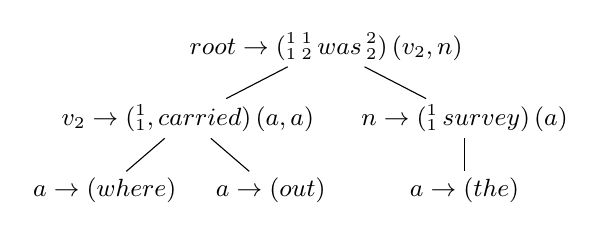
\begin{tikzpicture}[baseline=(v.base), level distance=6ex, font=\small, sibling distance=3.7cm, inner sep=2pt, level 2/.style={sibling distance=6em}, level 1/.style={sibling distance=10em}]
            \node (root) {\(\nt{root} \to (\x_1^1\,\x_2^1\,\tn{was}\,\x_2^2)\,(\nt{v}_2, \nt{n})\)}
            child {node (v) {\(\nt{v}_2 \to (\x_1^1, \tn{carried})\,(\nt{a}, \nt{a})\)}
                child {node {\( \nt{a} \to (\tn{where})\)}}
                child {node {\( \nt{a} \to (\tn{out})\)}}}
            child {node {\(\nt{n} \to (\x_1^1\, \tn{survey})\,(\nt{a})\)}
                child {node {\(\nt{a} \to (\tn{the})\)}}};
        \end{tikzpicture}
        \hfill
        \begin{minipage}{.4\linewidth}
            \subcaption{Projection \(\pi_{\abrv{lcfrs}}(d)\) into an \abrv{lcfrs} derivation.}
        \end{minipage}

        \vspace{1cm}

        \begin{minipage}{.35\linewidth}
            \subcaption{Projection \(\pi_{\abrv{dcp}}(d)\) into a \abrv{dcp} derivation.}
        \end{minipage}
        \hfill
        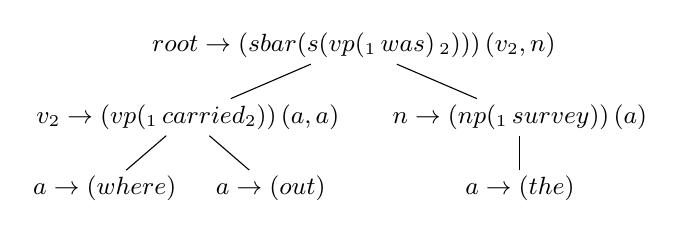
\begin{tikzpicture}[baseline=(v.base), level distance=6ex, font=\small, sibling distance=3.7cm, inner sep=2pt, level 2/.style={sibling distance=6em}, level 1/.style={sibling distance=12em}]
            \node (root) {\(\nt{root} \to (\cn{sbar} (\cn{s} (\cn{vp} (\x_1\, \tn{was})\,\x_2)))\,(\nt{v}_2, \nt{n})\)}
            child {node (v) {\(\nt{v}_2 \to (\cn{vp}(\x_1 \, \tn{carried} \x_2))\,(\nt{a}, \nt{a})\)}
                child {node {\( \nt{a} \to (\tn{where})\)}}
                child {node {\( \nt{a} \to (\tn{out})\)}}}
            child {node {\(\nt{n} \to (\cn{np} (\x_1 \, \tn{survey}))\,(\nt{a})\)}
                child {node {\(\nt{a} \to (\tn{the})\)}}};
        \end{tikzpicture}

        \vspace{1cm}

        \begin{tikzpicture}[baseline=(np.base), level distance=4ex, font=\small]
            \matrix (yields) [matrix of nodes, outer sep=0pt, inner sep=0pt, row sep=5ex, column sep=10pt] {
                \tn{where}\strut & \tn{carried}\strut & \tn{out}\strut & \tn{was}\strut & \tn{the}\strut & \tn{survey}\strut \\
                \tn{where}\strut  & \tn{the}\strut  & \tn{survey}\strut   & \tn{was}\strut  & \tn{carried}\strut  & \tn{out}\strut  \\};
            \node[above=15 ex of yields] (root) {\cn{sbar}}
            child {node {\cn{s}}
                child {node[above=7ex of yields-1-3] (vp1) {\cn{vp}}
                    child {node[above=3ex of yields-1-2] (vp2) {\cn{vp}}}}
                child {node[above=3ex of yields-1-5, xshift=4ex] (np) {\cn{np}}}};
            \draw (np) -- (yields-1-5) (np) -- (yields-1-6);
            \draw (vp1) -- (yields-1-4);
            \draw (vp2) -- (yields-1-1) (vp2) -- (yields-1-2) (vp2) -- (yields-1-3);
            \draw
                (yields-1-1.south) -- (yields-2-1.north)
                (yields-1-2.south) -- (yields-2-5.north)
                (yields-1-3.south) -- (yields-2-6.north)
                (yields-1-4.south) -- (yields-2-4.north)
                (yields-1-5.south) -- (yields-2-2.north)
                (yields-1-6.south) -- (yields-2-3.north);
        \end{tikzpicture}
    \hfill
        \begin{minipage}{.4\linewidth}
            \subcaption{\label{fig:hybrid:hybridtree}
                Hybrid tree for the derivation \(d\).
                The upper part is the yield for the \abrv{dcp} projection of \(d\), the bottom-most string is the yield for the \abrv{lcfrs} projection.
                The alignment between the lexical symbols is illustrated as paths between the leaf positions in the upper part and the positions in the bottom string.
            }
        \end{minipage}

        \vspace{.5cm}

        \caption{\label{fig:hybrid:derivation}
            The two projections for the \abrv{hg} derivation \(d\) shown in \cref{ex:hg:derivation} and an illustration of the resulting hybrid tree that combines the yield of both projections.
        }
    \end{figure}

    \begin{example}\label{ex:hg:derivation}
        Consider the following tuples of \abrv{lcfrs} and \abrv{dcp} compositions
        \begin{align*}
            c_1 &= (\tn{where})\;(\tn{where}),
            &c_2 &= (\tn{the})\;(\tn{the}),
            &c_3 &= (\tn{out})\;(\tn{out}), \\
%
            c_4 &= (\x_1^1\, \tn{survey})\;(\cn{np} (\x_1 \, \tn{survey})), \\
            c_5 &= (\x_1^1, \tn{carried}\,\x_2^1)\;(\cn{vp}(\x_1 \, \tn{carried} \x_2)), \\
            c_6 &= (\x_1^1\,\x_2^1\,\tn{was}\,\x_2^2)\;(\cn{sbar} (\cn{s} (\cn{vp} (\x_1\, \tn{was})\,\x_2)))
        \end{align*}
        and the \abrv{hg} \(G= (\{\nt{root}, \nt{v}_2, \nt{n}, \nt{a}\}, \Gamma, \Sigma, \nt{root}, R)\) over the alphabets \(\Gamma = \{\cn{sbar}, \cn{s}, \cn{vp}, \cn{np}\}\) and \(\Sigma = \{\tn{where}, \tn{the}, \tn{survey}, \tn{was}, \tn{carried}, \tn{out}\}\), and with the following rules:
        \begin{align*}
            \nt{root} &\to c_6 (\nt{v}_2, \nt{n}), & \nt{v}_2 &\to c_5 (\nt{a}, \nt{a}), & \nt{n} &\to c_4 (\nt{a}), \\
            \nt{a} &\to c_1, & \nt{a} &\to c_2, & \nt{a} &\to c_3
        \end{align*}

        \noindent
        \begin{minipage}[t]{.65\linewidth}
            The figure to the right illustrates a derivation \(d\) in \(G\).
            The two projections \(\pi_{\abrv{lcfrs}}(d)\) and \(\pi_{\abrv{dcp}}(d)\) are shown in \cref{fig:hybrid:derivation}.
            The yield of \(d\) is understood as a combination of both projections' yields with aligned leaf and string positions as shown in \cref{fig:hybrid:hybridtree}.
            The illustrated hybrid tree is equivalent to the constituent structure and token sequence shown in \cref{fig:pre:ctree}.
        \end{minipage}
        \hfill
        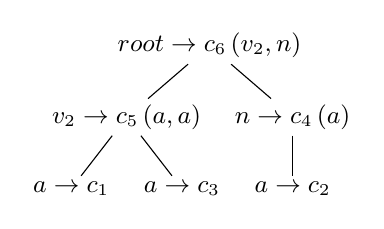
\begin{tikzpicture}[baseline=(root.base), level distance=6ex, font=\small, inner sep=2pt, level 2/.style={sibling distance=4em}, level 1/.style={sibling distance=6em}]
            \node (root) {\(\nt{root} \to c_6\,(\nt{v}_2, \nt{n})\)}
            child {node {\(\nt{v}_2 \to c_5\,(\nt{a}, \nt{a})\)}
                child {node {\( \nt{a} \to c_1\)}}
                child {node {\( \nt{a} \to c_3\)}}}
            child {node {\(\nt{n} \to c_4\,(\nt{a})\)}
                child {node {\(\nt{a} \to c_2\)}}};
        \end{tikzpicture}
    \end{example}

    In a position instantiated \abrv{hg}, each pair of lexical symbols is replaced by the same position.
    A derivation is called \emph{admissible} if its \abrv{lcfrs} projection is admissible.
    In the case of an admissible position instantiated derivation, the concept of alignments between lexical symbols is superfluous, as each position must occur at most once (synchronously in a tuple of compositions).
    The constituent structure for such a derivation coincides with the yield of the \abrv{dcp} projection.

    \vspace{\baselineskip}

    \noindent
    \begin{minipage}{.4\linewidth}
        \begin{example}
            The figure to the right illustrates a position instance for the derivation \(d\) (cf.\@ \cref{ex:hg:derivation}) in the sequence of tokens ``where the survey was carried out''.
            It is an admissible derivation, i.e.\@ the yield of the string projection is the sequence of consecutive positions from 1 to 6.
            The constituent structure is one of our running examples, as seen in \cref{ex:dcp:comp}.
        \end{example}
    \end{minipage}
        \hfill
    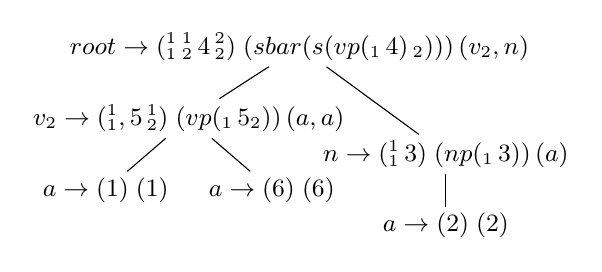
\begin{tikzpicture}[baseline=(n.north),level distance=6ex, font=\small, inner sep=2pt, level 2/.style={sibling distance=6em}, level 1/.style={sibling distance=8em}]
        \node (root) {\(\nt{root} \to (\x_1^1\,\x_2^1\,\tn{4}\,\x_2^2)\;(\cn{sbar} (\cn{s} (\cn{vp} (\x_1\, \tn{4})\,\x_2)))\,(\nt{v}_2, \nt{n})\)}
        child {node (v) {\(\nt{v}_2 \to (\x_1^1, \tn{5}\,\x_2^1)\;(\cn{vp}(\x_1 \, \tn{5} \x_2)) \,(\nt{a}, \nt{a})\)}
            child {node {\( \nt{a} \to (\tn{1})\;(\tn{1})\)}}
            child {node {\( \nt{a} \to (\tn{6})\;(\tn{6})\)}}}
        child {node[yshift=-3ex, xshift=3ex] (n) {\(\nt{n} \to (\x_1^1\, \tn{3})\;(\cn{np} (\x_1 \, \tn{3}))\,(\nt{a})\)}
            child {node {\(\nt{a} \to (\tn{2})\;(\tn{2})\)}}};
    \end{tikzpicture}
\end{document}